\chapter{Implementation and Result Analysis}

\section{Introduction}
This chapter demonstrates the implementation and result analysis of the Voice Search Chrome Extension. This chapter describes the  technologies are used here to develop, development details with code snippet, testing strategies and performance evaluation of the system. Screenshot and tables are included to show the functionalities and performance of the project.

The primary goal of this chapter is to show how the methodology proposed in the Chapter 3 has been implemented into a working software product. The result highlights the efficiency, accuracy and usability of the extension.



\section{Technologies Used and Their Application}
Table 4.1 demonstrates each technology used here to ensure performance, modularity and accessibility.
\begin{table}[H]
\centering
\caption{Technologies Used and Their Application}
\label{tab:technologies_used}
\begin{tabular}{|p{4cm}|p{10cm}|}
\hline
\textbf{Technology} & \textbf{Purpose / How It Was Used} \\ \hline
JavaScript (ES5) & Used to implement core logic for capturing voice, parsing commands, executing browser actions \\ \hline
Chrome Extension APIs & Used for tab management, content scripts, and browser interaction \\ \hline
Web Speech API & Converts voice input to text and detects language (English/Bengali). \\ \hline
JSON & Stores commands and mappings to the corresponding actions \\ \hline
HTML / CSS & used for designing Floating mic button and UI for feedback \\ \hline

\end{tabular}
\end{table}


\section{Implementation Details and Results}

\subsection{Voice Input Process}
Voice Input Process deals with the receiving voice commands from the users and converts them into text and pass for next stage. This process is implemented in core.js. Browser SpeechRecognition API is used to capture user voice input. The speech recognition object initialized with continuous listening and interim results for speech-to-text conversion.


\begin{minted}[
  frame=single,
  framesep=5pt,
  linenos,
  autogobble
]{javascript}
recognition = new SpeechRecognition();
recognition.lang = window.selectedLanguageCode || "en-US";
recognition.continuous = true;
recognition.interimResults = true;
\end{minted}
The system reacts to different events. \textit{onstart} - used for activating mic icon provide indication that mic is under listening mode. \textit{onerror/onend} is used to stop recognition if errors or silence occur. \textit{onresult} event sends recognized text to \textit{handleRecognitionResult} function.
\begin{minted}[
  fontsize=\small,
  frame=single,
  framesep=5pt,
  linenos,
  autogobble, breaklines
]{javascript}
recognition.onstart = () => {
    document.getElementById("floating-mic").style.background = "#28a745";
    showBubble("�� Listening...");
  };

  recognition.onerror = (e) => {
    stopRecognition();
    showBubble("❌ Error: " + e.error);
  };

  recognition.onend = () => {
    document.getElementById("floating-mic").style.background = "#007bff";
  };

  recognition.onresult = handleRecognitionResult;
\end{minted}
The function \textit{handleRecognitionResult} checks transcript, match predefined command and execute corresponding browser action(e.g scroll, open site, media control). 
\begin{minted}[
  fontsize=\small,
  frame=single,
  framesep=5pt,
  linenos,
  autogobble, breaklines
]{javascript}
function handleRecognitionResult(event) {
  ......
  for (let i = event.resultIndex; i < event.results.length; i++) {
    const result = event.results[i];
    const transcript = result[0].transcript.trim().toLowerCase();
    const isFinal = result.isFinal;
    if (!transcript) continue;
    showBubble(isFinal ? "��️ " + transcript : "…" + transcript);
    const match = matchCommand(transcript);
    ......
\end{minted}
\subsubsection*{Screenshot}
\begin{figure}[htbp] 
    \centering
    \fbox{%
    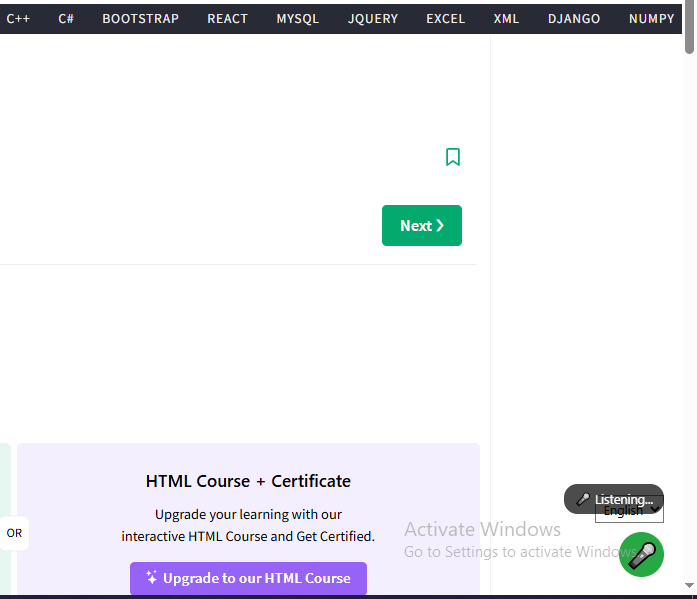
\includegraphics[width=0.7\textwidth, height=0.7\textheight, keepaspectratio]{latex/Chap4/4.3.1.listening.png}
    }
    \caption{ Active mic with “Listening...” bubble.}
    \label{fig:active_mic}
\end{figure}

Figure 4.1 displays the visual feedback of listening mic. It shows that it is ready to take voice input.

\subsection{Media Control}

The Media Control module used for voice-based interaction with video element of the page. 
Once the user says \textit{``start media''}, the system enable Media Mode to allow media commands such as play, pause, volume up/down etc. 

After matching the intent, detected commands are executed on the active \texttt{<video>} element and feedback is displayed on-screen speech transcript.

\begin{minted}[fontsize=\small,
  frame=single,
  framesep=5pt,
  linenos,
  autogobble, breaklines]{javascript}
// Enabling and disabling Media Mode
if (intent === "start_media") {
   mediaMode = true;
   showBubble("Media mode enabled");
}
if (intent === "stop_media") {
   mediaMode = false;
   showBubble("Media mode disabled");
}
// Passing commands to media.js
if (mediaMode && intent.startsWith("media_")) {
   handleMediaCommand(intent, value);
}
\end{minted}

In \texttt{media.js}, \texttt{handleMediaCommand()} function handle different video actions. For example, when user speak "play" video will start and when user say "pause" video will pause(shown in 2 to 10 lines). The following examples illustrate how commands are executed:

\begin{minted}[fontsize=\small,
  frame=single,
  framesep=5pt,
  linenos,
  autogobble, breaklines]{javascript}
// Playing a video
case "media_play":
   video.play();
   showBubble("Playing");
   break;
// Pausing a video
case "media_pause":
   video.pause();
   showBubble("Paused");  // visual transcript
   break;
// Other commands in similar fashion...
\end{minted}

These code snippets shows the way to map different voice commands 
to execute actions, enable consuming media content almost hands completely hands-free for users.
\subsubsection*{Screenshot}
\begin{figure}[htbp] 
    \centering
    \fbox{%
    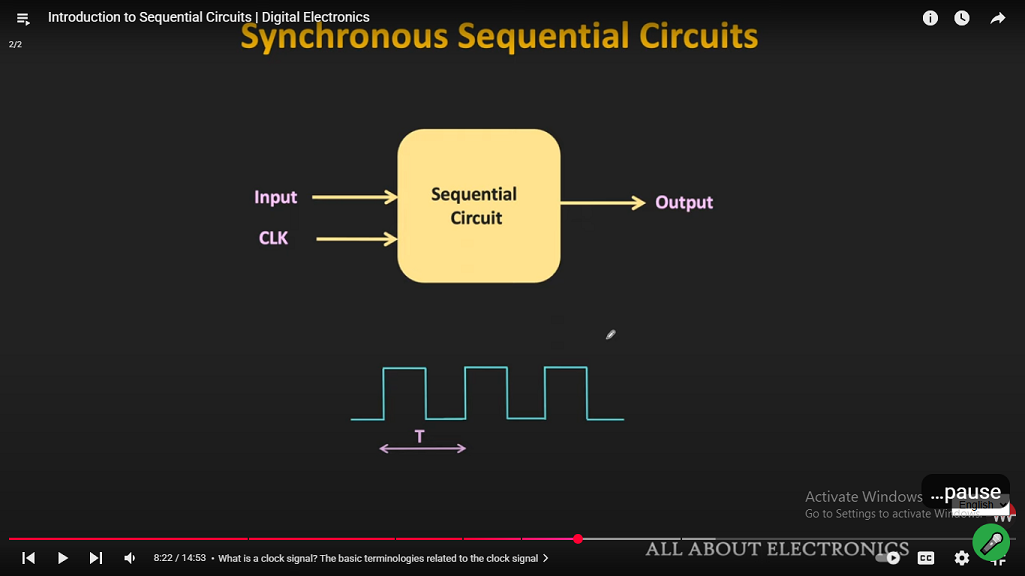
\includegraphics[width=1\textwidth, height=0.7\textheight, keepaspectratio]{latex/Chap4/4.3.2.pause.png}
    }
    \caption{ Pause the media content through voice}
    \label{fig:pause_media}
\end{figure}

Figure 4.2 refers that, a visual display of pausing a media content by "pause" command.

\subsection{Tab Management}
This extension provides voice-controlled tab management features. It allows to users to control the browser tabs without manual interaction. It supports opening new sites of name or opening new tab, switching between tabs, view all the tabs in list of current window and closing active window through voice command. Sample examples of voice commands to access these features are given below:

\subsubsection*{Example commands:}
\begin{itemize}
    \item \texttt{"open YouTube"}: Opens \texttt{youtube.com} in a new tab.
    \item \texttt{"next tab"}: Switches to the next tab in the browser.
    \item \texttt{"previous tab"}: Switches to the previous tab.
    \item \texttt{"switch to [title]"}: Finds the title by matching the phrase after saying "switch to". 
    \item \texttt{"close tab"}: Closes the currently active tab.
    \item  \text{"show tab"}: Displays a popup window with all open tabs.
\end{itemize}

The workflow is described as user commands are recognized by the speech recognition module, then matched to intents such as \texttt{open\_site}, \texttt{tab\_next}, \texttt{tab\_previous}, or \texttt{tab\_close}.After that it sends to message to background.js file. It communicates with the Chrome Tabs API to perform the actual tab operations.

In below code describes how message is sent from core.js after matching the intent to the background.js file which executes the following tab operation.

\begin{minted}[frame=single,framesep=5pt,linenos,autogobble]{javascript}
// core.js (user says "switch to youtube")
if (intent === "tab_switch") {
  chrome.runtime.sendMessage({
    action: "switch_tab",
    query: value,   // e.g., "youtube"
  });
}
\end{minted}

\begin{minted}[frame=single,framesep=5pt,linenos,autogobble, breaklines]{javascript}
// Example: Switching to a tab by title
if (msg.action === "switch_tab") {
  const query = msg.query;
  chrome.tabs.query({ currentWindow: true }, function (tabs) {
    for (let i = 0; i < tabs.length; i++) {
      if (tabs[i].title.toLowerCase().includes(query.toLowerCase())) {
        chrome.tabs.update(tabs[i].id, { active: true });
        break; } } }); }
\end{minted}

This tab management module provides better accessibility to users  through the browser without manual interaction every time.

\subsubsection*{Screenshot:}
\begin{figure}[htbp] 
    \centering
    \fbox{%
    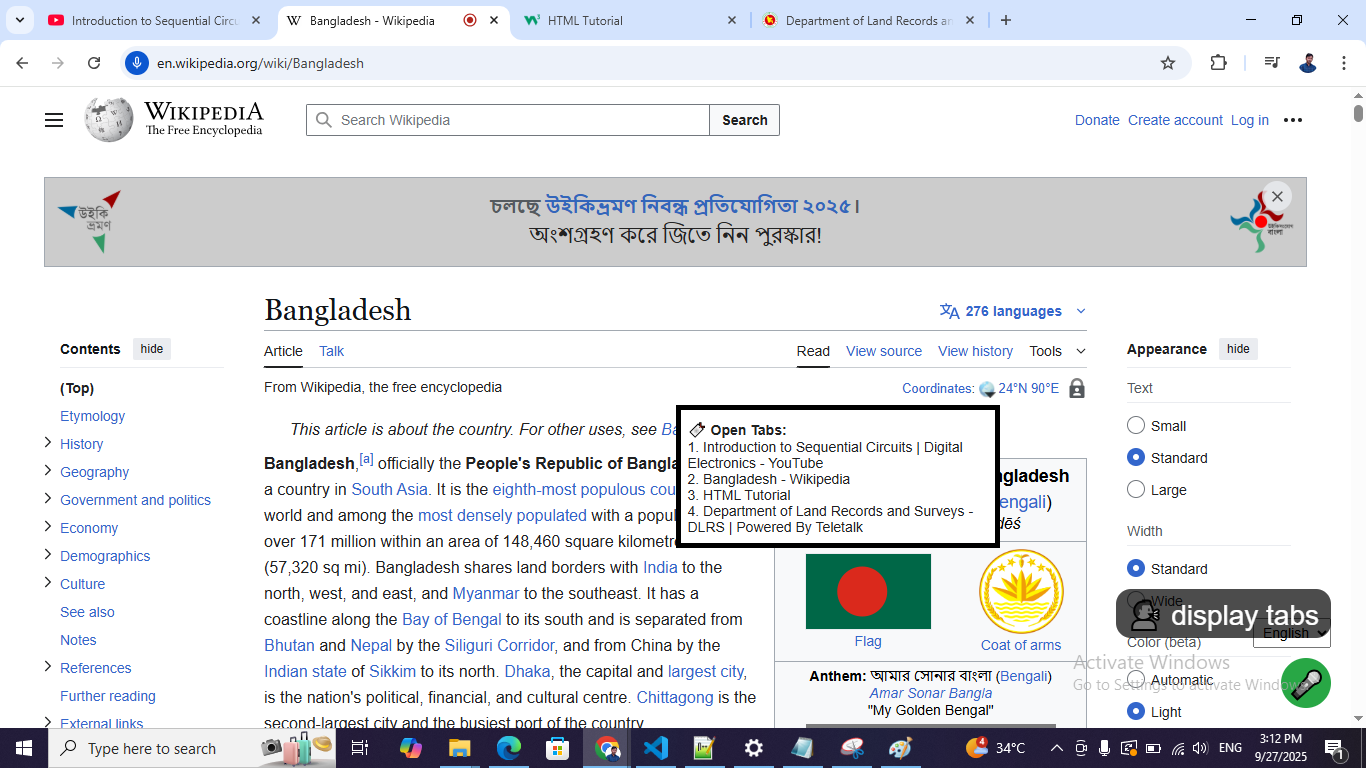
\includegraphics[width=0.7\textwidth, height=0.7\textheight, keepaspectratio]{latex/Chap4/4.3.3.tab_management.png}
    }
    \caption{ Display existing tab list of current window}
    \label{fig:display_tabs}
\end{figure}

Figure 4.3 displays the list of opening tabs in current window by speaking "display" command.

\subsection{Scrolling and Zooming}
This feature allows users to scroll up/down the current page.Users can also set/reset zoom level through voice commands. For achieving this feature, user can perform following commands such as \texttt{scroll\_up}, \texttt{scroll\_down}, \texttt{scroll\_top}(scroll to the very top position), \texttt{scroll\_last}(scroll at the bottom of the page), \texttt{zoom\_in}, \texttt{zoom\_out}, \texttt{reset\_zoom}(to reset the zoom level to 100%). 
In below code, it shown that how "scroll up" and "zoom in" command execute those actions.

\begin{minted}[frame=single, framesep=5pt, linenos, autogobble]{javascript}
// Scroll down by 400px
if (intent === "scroll_down") window.scrollBy(0, 400);

// Zoom in by increasing current zoom step
if (intent === "zoom_in") {
    currentZoom = Math.min(currentZoom + ZOOM_STEP, 2);
    document.body.style.zoom = currentZoom;
    showBubble(`Zoomed in to ${Math.round(currentZoom * 100)}%`);
}
\end{minted}

\vspace{1in} 

\textbf{Screenshot:}

\begin{figure}[H] 
    \centering
    \fbox{%
    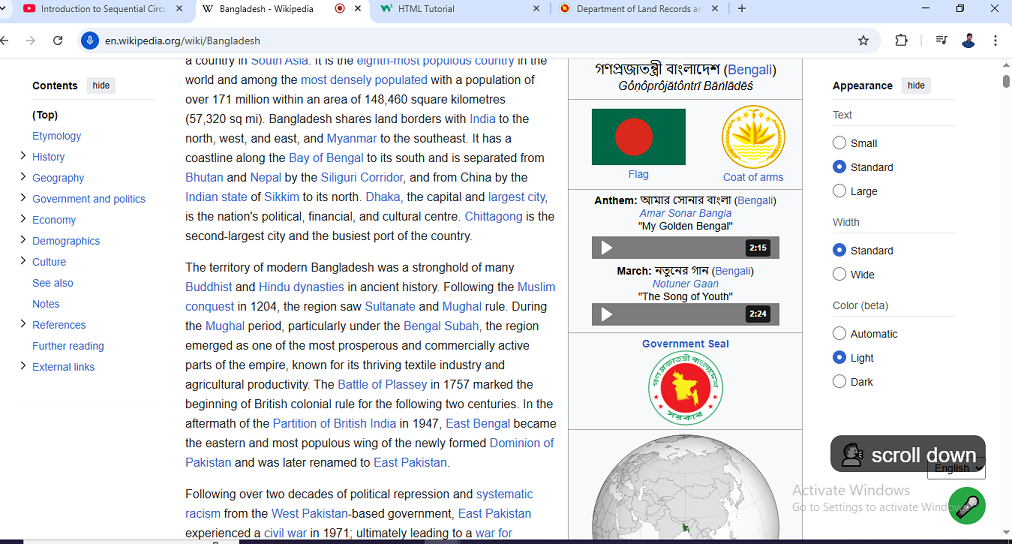
\includegraphics[width=0.8\textwidth, height=0.8\textheight, keepaspectratio]{latex/Chap4/4.3.4.scroll_down.png}
    }
    \caption{Scroll down through voice}
    \label{fig:scroll_down}
\end{figure}

Figure 4.4 shows a screenshot of scrolling down a webpage.

\subsection{Link Interaction}
This feature enables users to highlight and click links by title on the webpage using voice commands for easier navigation. Available intents and sample commands are given below:

\begin{itemize}
    \item \texttt{show\_links}: ``show links'', ``highlight links''
    \item \texttt{click\_link}: ``click Facebook'', ``link Gmail''
    \item \texttt{hide\_links}: ``hide links'', ``remove links''
\end{itemize}

here user can click the link by saying numbers which are highlighted 
after executing \texttt{show\_links} or by saying inner text of any hyperlink.The code sample of how user can click link by title is given below:

In the below code, from 3-4 lines, it finds out the matching hyperlink from the collected hyperlink list \texttt{cachedLinks}. From 6-10, if there is any match then,it highlights the link with yellow color and click the link. Visual feedback will be provided if there is no match with title, are shown in number 11-13 lines. 

\vspace{1in}

\begin{minted}[frame=single, framesep=5pt, linenos, autogobble]{javascript}
// Find and click a link whose text contains the given title
function clickLinkByTitle(title) {
    const match = cachedLinks.find((l) =>
      l.innerText.toLowerCase().includes(title.toLowerCase())
    );
    if (match) {
        match.scrollIntoView({ behavior: "smooth", block: "center" });
        match.style.background = "yellow"; // temporary highlight
        setTimeout(() => match.click(), 600);}}
\end{minted}


% Placeholder for screenshot
\textbf{Screenshot:}

\begin{figure}[htbp] 
    \centering
    \fbox{%
    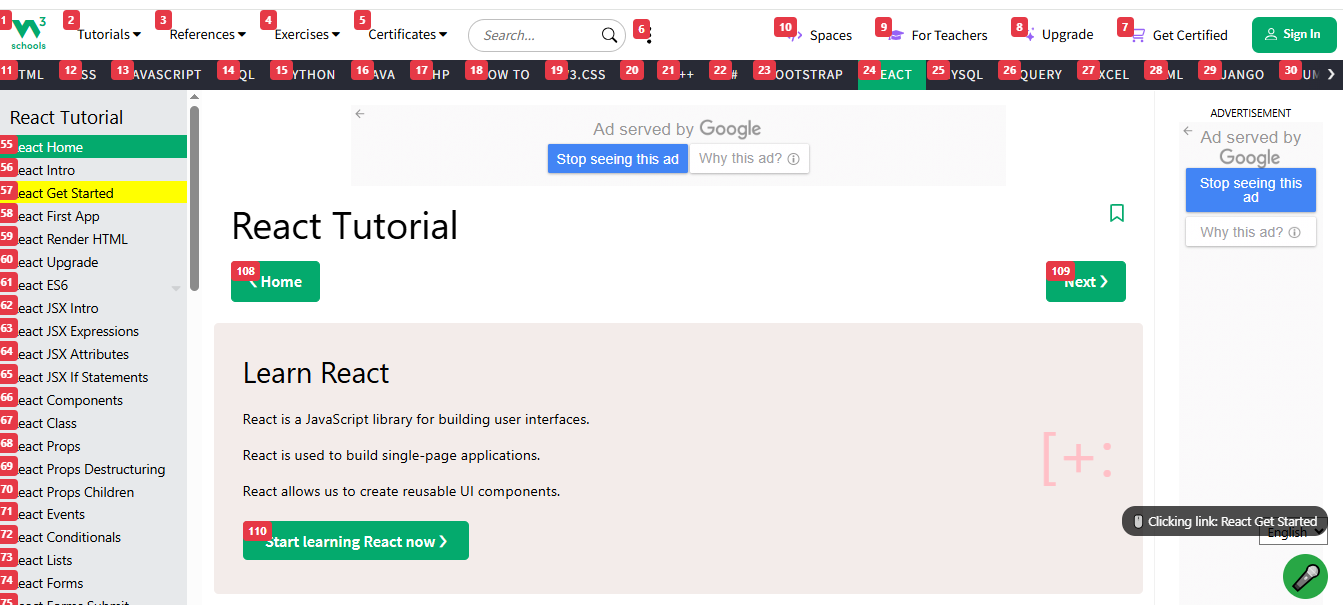
\includegraphics[width=0.8\textwidth, height=0.8\textheight, keepaspectratio]{latex/Chap4/4.3.5.highlight_links.png}
    }
    \caption{Click link by title from the highlighted links}
    \label{fig:click_highlight_links}
\end{figure}

Figure 4.5 displays a screenshot of all the available links with numbered badges in a webpage. 

\subsection{Reading Selected Text}
This feature is designed to improve the accessibility of extension by enabling read aloud webpage content. User can start this feature by voice command such as "start reading". Once activated, the readable sections of the webpage(paragraph, list) are highlighted through numbers.
Later, user can read those particular section by selecting the selection by number. The selected content is displayed in a dedicated pop up window and starts reading until finishing the content.
\subsubsection*{Available Commands}
\begin{itemize}
    \item \texttt{Start Reading}: User can highlight readable sections with assigns numbers.  
    \item \texttt{Read by Number [X]}: This command opens a pop up window containing the selected section by number and starts reading.
    \item \texttt{Stop Reading}: This command stops ongoing reading and closes the popup window.  
    \item \texttt{Clear Highlights}: This command is used for removing number badges from the section and borders from the page.  
\end{itemize}

\textbf{Implementation}

After triggering reading mode, \texttt{highlightReadableSections()} scans whole webpage and collect <p>, <ol> and <ul> sections.
\begin{minted}[frame=single, framesep=5pt, linenos, autogobble,breaklines]{javascript}
//
function highlightReadableSections() {
  const sections = document.querySelectorAll("p, ol, ul");
  ......
  });

  showBubble("Numbered readable sections");
}
\end{minted}

Then if user says "read number 3", then selected content is loaded by \texttt{readSectionByNumber()} 
 in pop up window starts reading the text using \texttt{startReadingSectionFromPopup} function.

\begin{minted}[frame=single, fontsize=\small, linenos]{javascript}
function readSectionByNumber(number) {
  const el = document.querySelector(`[data-read-id="${number}"]`);
  if (!el) return;
  const text = el.innerText.trim();
  showReadPopup(number, text); 
  startReadingSectionFromPopup(text); 
}
\end{minted}

\vspace{1in}

\begin{minted}[frame=single, fontsize=\small, linenos]{javascript}
function startReadingSectionFromPopup(text) {
  currentReadSentences = splitIntoSentences(text);
  currentReadSentences.forEach((s,i) => {
    const span = document.createElement("span");
    span.innerText = s + " ";
    span.dataset.index = i;
    content.appendChild(span);
  });  speakNextSentence(); }
\end{minted}


 After loading into popup window entire text is divided into sentences by function \texttt{splitIntoSentences()}.Then Browser SpeechSynthesis API reads each word sequentially by \texttt{speakNextSentence()} function. While reading each sentence is highlighted with yellow color. After finishing reading, popup window will be closed automatically.

 
\begin{minted}[frame=single, fontsize=\small, linenos]{javascript}
function speakNextSentence() {
  if (currentReadIndex >= currentReadSentences.length) return;
  const sentence = currentReadSentences[currentReadIndex];
  const u = new SpeechSynthesisUtterance(sentence);
  u.onstart = () => highlightSentence(currentReadIndex);
  u.onend   = () => { currentReadIndex++; speakNextSentence(); };
  window.speechSynthesis.speak(u);
}
\end{minted}

\subsubsection*{Screenshots:}

\begin{figure}[H] 
    \centering
    \fbox{%
    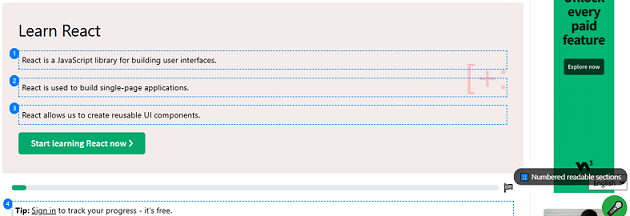
\includegraphics[width=0.8\textwidth, height=0.8\textheight, keepaspectratio]{latex/Chap4/4.3.6.1.highlight_readable_section.png}
    }
    \caption{Highlighted readable section with numeric badges}
    \label{fig:highlighted_readable_section}
\end{figure}

Figure 4.6 displays a screenshot of highlighted readable section of current webpage

\begin{figure}[H] 
    \centering
    \fbox{%
    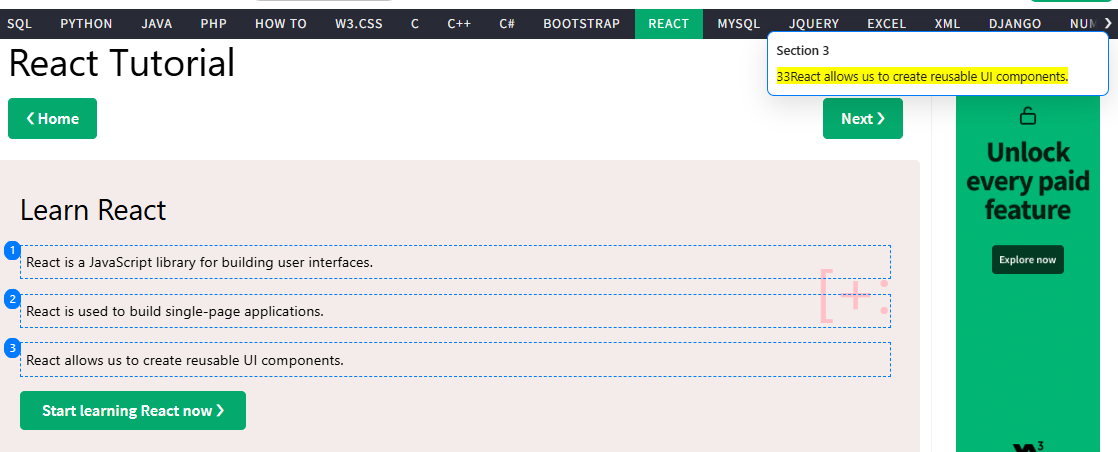
\includegraphics[width=0.8\textwidth, height=0.8\textheight, keepaspectratio]{latex/Chap4/4.3.6.2.read_from_section.png}
    }
    \caption{Read a loud from selected section in popup window}
    \label{fig:read_loud_selected_section}
\end{figure}

Figure 4.7 illustrates the voice narration of a selected section. It shows that a pop up window is appeared and highlighted text is spoken by speech API.

There is another way to implement this feature. Context menu is added here to read both English and Bengali language. User needs to select text and click context menu option from the right menu. By this way, it can read selected text loudly. Here is a screenshot of this activity.

\begin{figure}[H] 
    \centering
    \fbox{%
    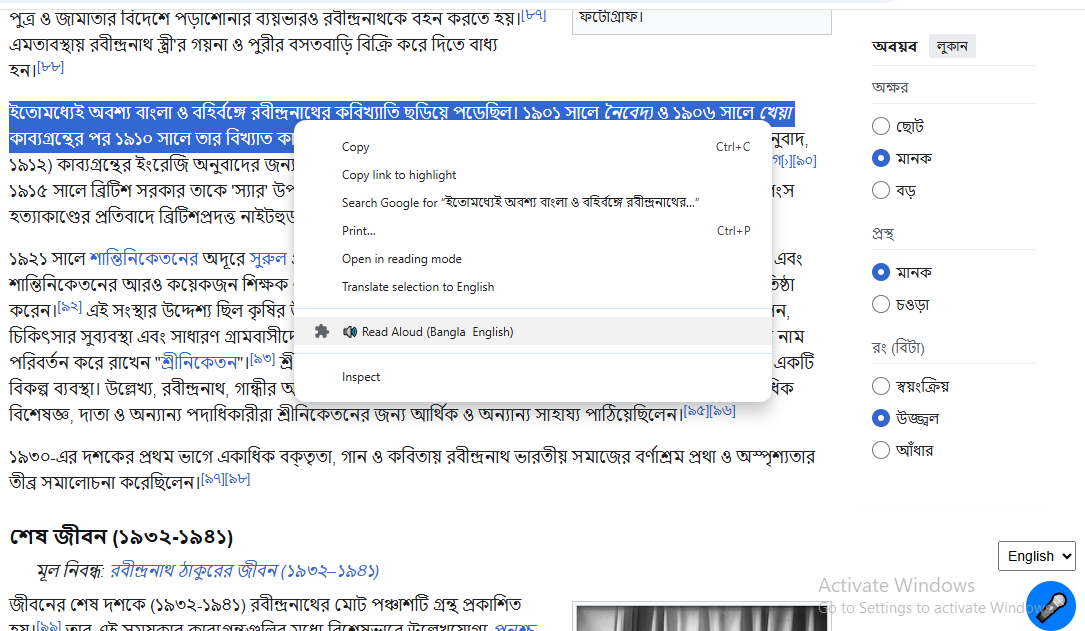
\includegraphics[width=0.8\textwidth, height=0.8\textheight, keepaspectratio]{latex/Chap4/4.3.6.3.bangla_reading.png}
    }
    \caption{Read a loud from selected Bengali text}
    \label{fig:read_loud_selected_section}
\end{figure}

Figure 4.8 displays a screenshot of reading Bengali text by selecting right menu.

\subsection{Voice-Controlled Form Fill-Up}
The Form Fill-Up feature enables user to fill the form without manual interaction, User can fill the form through voice. Right now this feature only supports English language only.

\subsubsection*{Available Commands:}

\begin{itemize}
    \item \textbf{Mode Control:} \texttt{start_form} is used to enable form mode, so that after this each commands executed for form purpose. \texttt{stop_form} is used for exit from the form mode.
    \item \textbf{Navigation:} User can use \texttt{next}, \texttt{reverse}, \texttt{back} commands to go back the previous field. User can also navigating by saying index number.
    \item \textbf{Input Handling:} Spoken words are filled into the active field; \texttt{clear} command is used to clear the active field. There is a option to fill up the password field by the secure password suggestion with \texttt{yes}/\texttt{no}. Dropdown control using \texttt{down}, \texttt{up}, or \texttt{option 3}; radio button selection can be done by saying \texttt{select male}, \texttt{choose female}.
    \item \textbf{Submission:} User can submit the form by saying \texttt{"submit form"}, \texttt{"form done"}.
\end{itemize}

\subsubsection*{System Workflow:}

The overall form handling process can be summarized as follows:
\paragraph{1. Activate Form Mode:}
When the user says \textit{``start form''}, all form fields like (\texttt{input}, \texttt{textarea}, \texttt{select}) are collected and the first field of the form is focused.

\begin{minted}[fontsize=\small,
  frame=single,
  framesep=5pt,
  linenos,
  autogobble, breaklines]{javascript}
formFields = Array.from(
    document.querySelectorAll("input, textarea, select")
).filter((el) => el.offsetParent !== null && !el.disabled);
formFields[currentFieldIndex].focus();
\end{minted}

\subsubsection*{Screenshot:}
\begin{figure}[H] 
    \centering
    \fbox{%
    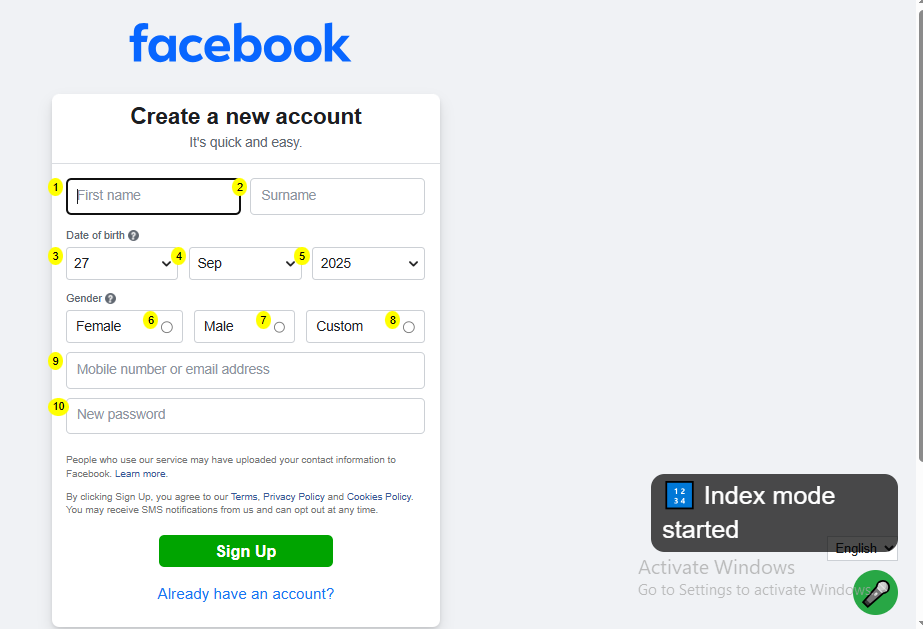
\includegraphics[width=0.7\textwidth, height=0.7\textheight, keepaspectratio]{latex/Chap4/4.3.7.form_index.png}
    }
    \caption{Start form mode with index number to each field}
    \label{fig:start_form}
\end{figure}

Figure 4.9 shows the visual display of a indexed form fields of Facebook login page. When user speaks "start form" first field of form is focused and index number is added to each field of the form. 

\paragraph{2. Navigate Between Fields:}
Users can move forward/backward in the form using \texttt{next} or \texttt{reverse}. Each navigation updates the field's current index and focuses to the new field.

\begin{minted}[fontsize=\small,
  frame=single,
  framesep=5pt,
  linenos,
  autogobble, breaklines]{javascript}
case "form_next":
  currentFieldIndex++;
  formFields[currentFieldIndex].focus();
  showBubble("➡️ Moved to next field");
\end{minted}

\paragraph{3. Input Processing:}
After second step, spoken text said by user is typed into the active field. Passwords can be filled by password suggestions and drop downs are handled by different commands.

\begin{minted}[fontsize=\small,
  frame=single,
  framesep=5pt,
  linenos,
  autogobble, breaklines]{javascript}
function handleGeneralInput(transcript, field) {
  field.value = transcript;
  showBubble("✏️ Typed: " + transcript);
}
\end{minted}

\paragraph{4. Form Submission:}
After filling up forms, if the user says \textit{``submit form''}, the system detects the form and submit the form.

\begin{minted}[fontsize=\small,
  frame=single,
  framesep=5pt,
  linenos,
  autogobble, breaklines]{javascript}
const btn = form.querySelector("button[type='submit']");
if (btn) { btn.click(); }
else { form.submit(); }
showBubble("✅ Form submitted");
\end{minted}

\subsection{Inline Search}
In this feature, user can search from google or youtube by speaking phrase. if current url is youtube, it will search in youtube otherwise the phrase term is searched in google.

When user speaks \texttt{"search some_text"}, function \texttt{isGoogleSearchPage()} or \texttt{isYouTubeSearchPage()} is called to find out the current url, later phrase is submitted by the google or youtube search bx.

\begin{minted}[fontsize=\small,
  frame=single,
  framesep=5pt,
  linenos,
  autogobble, breaklines]{javascript}
function isGoogleSearchPage() {
  return (
    location.hostname.includes("google") &&
    document.querySelector("textarea[name='q']")
  );
}

if (isGoogleSearchPage()) {
    input = document.querySelector("textarea[name='q']");
  }

  if (input) {
    input.value = query;
    input.dispatchEvent(new Event("input", { bubbles: true }));
}
\end{minted}

\subsubsection*{Screenshot:}
\begin{figure}[H] 
    \centering
    \fbox{%
    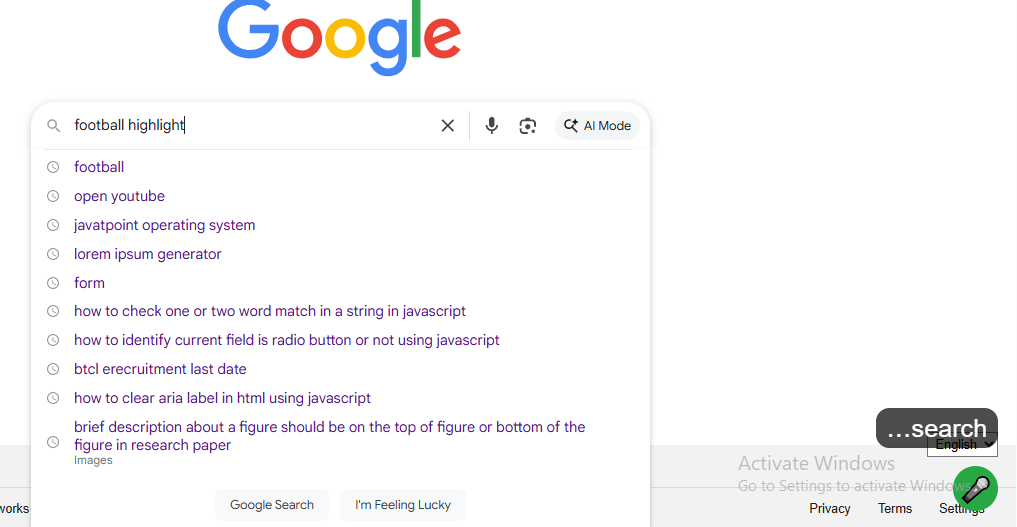
\includegraphics[width=0.7\textwidth, height=0.7\textheight, keepaspectratio]{latex/Chap4/4.3.8.inline_search.png}
    }
    \caption{Inline search in Google through voice}
    \label{fig:inline_search}
\end{figure}

Figure 4.10 represents a screenshot of hands free voice search through Google.

\section{Testing and Result Analysis}
\begin{itemize}
\item	Functional Testing: In this test the system shows majority of the features works as expected like search commands, tab control, inline search, media control.
\item	Performance Testing: Measures response time from voice input to command action. It reflects the average time to perform any task. In this section, accuracy of the recognition and scalability are also checked. 
\item	Language Testing: In this test, checks the language is detected successfully, toggling language is worked, and voice command in both languages works just as fine majority time.
\item	Cross-page Testing: Cross functionality check is perform on different websites(Google, Youtube, Facebook etc.)
\end{itemize}


Table 4.2 shows that the test results for each feature included in extension. It detect the accuracy of the features by depicting pass/fail and response time for each item.

\begin{table}[H]
    \centering
    \caption{Feature vs. Test Result Evaluation\cite{voiceweb_test_results}}
    \label{tab:feature_test_results_professional}
    \begin{tabularx}{\textwidth}{>{\RaggedRight\arraybackslash}X c r}
        \toprule
        \textbf{Feature / Test Type} & \textbf{Status} & \textbf{Avg. Response Time (ms)} \\
        \midrule
        Voice-based Search                  & \textcolor{green!70!black}{Pass} & 350 \\ 
        Tab Control                         & \textcolor{green!70!black}{Pass} & 140 \\ 
        Form Filling                        & \textcolor{orange!80!black}{Pass (minor issue)} & 3.5 \\ 
        Media Control                     & \textcolor{green!70!black}{Pass} & 2 \\  
        Click Links by Number/title      &   
        \textcolor{green!70!black}{Pass} & 2.0 \\
        Inline Search                    &   \textcolor{green!70!black}{Pass} & 2.1 \\
        Language Toggle                     & \textcolor{green!70!black}{Pass} &  2 \\
        Cross-page Testing (Google, YouTube, Facebook) & \textcolor{green!70!black}{Pass} & 2 \\
        Recognition Accuracy                & \textcolor{blue!70!black}{80--85\% (Majority Pass)} & 1 \\
        \bottomrule
    \end{tabularx}
\end{table}


\section{Conclusion}
Chapter 4 detailed the implementation and the result analysis of the proposed system. This chapter covers both logical and physical design, technologies used, key features of the system. Also screenshots and performance and result tests confirm that the system provides responsiveness, scalability, accuracy and multilingual support. The result shows that the system is successfully translated from the proposed methodology and ready to enhance its features in future.






